\providecommand{\main}{../main}
\documentclass[\main/main.tex]{subfiles}
\graphicspath{{../images/}}
\begin{document}
\section{
    双対変換とダイマー模型
}
\begin{frame}{\currentname}
    QDMをゲージ理論の見方から解析する。
    古典的な背景場$B(e)$によって、
    \begin{align}
        E(e) = ∂N(e) + B(e)
    \end{align}
    と表す。$N(e)$は整数値を固有値にもつ演算子である。
    $B(e)$は
    \begin{align}
        ∂E(v) = ∂B(v) = ρ(v),␣
        ρ = ∑v_A - ∑v_B
    \end{align}
    を満たす。
    $B(e)$の設定には以下のような自由度がある。
    \begin{align}
        B(e) → B(e) - ∂S(e),␣ N(f) → N(f) + S(f)
    \end{align}
    コサイクル$\~γ_i$に対し、
    $(\~γ_i,B)$は$B$の取り方によらない不変量となる。
    $B$はサイクルではないので、$B$はホモロジー類をなさないことに注意。

    格子の双対変換をすると、$∂ ↔ \~∂$と置き換えることができる。
    すると$B(e)$はゲージ場に対応し、$N(v)$は物質場に対応する。
    また
    \begin{align}
        \~∂B(f) = ρ(f)
    \end{align}
    となり、$ρ$は電荷ではなく磁束になる。
\end{frame}
\begin{frame}{\currentname}
    $A(e)$と$E(e)$の間の正準交換関係から
    \begin{align}
        [(∂f,A),(e,E)] = ¡(e,∂f)
    \end{align}
    が成り立つ。
    $E = ∂N + B$を代入し、Stokesの定理を用いると
    \begin{align}
        [(f,\~∂A),(\~∂e,N)] = ¡(f,\~∂e)
    \end{align}
    となる。$B$が演算子でないことに注意。
    よって$N(f)$と$F(f) ≔ \~∂A(f)$の間に正準交換関係
    \begin{align}
        [F(f),N(f')] = ¡δ_{f,f'}
    \end{align}
    が設定される。
    $N(f)$は電磁場$F(f)$をシフトする演算子である。
\end{frame}
\begin{frame}{\currentname}
    QDMのハミルトニアン
    \begin{align}
        H = ÷{1}{2k}(‖E‖²-÷{|𝒱|}{2})
        + 2\=J∑_f \cos(\~∂A(f))
        + ÷{V}{2}‖\~∂E‖² - ÷{V|𝒱|}{2}
        \label{eq: H of QDM}
    \end{align}
    を双対な変数$B(e),N(f),F(f)$で表すと、
        \begin{align}
        H = ÷{1}{2k}(‖∂N+B‖²-÷{|𝒱|}{2})
        - 2\=J∑_v\cos F(v)
        + ÷{V}{2}‖-𝛥N + \~∂B‖² - ÷{V|𝒱|}{2}
        \label{eq: H of dual QDM}
    \end{align}
    となる。ただし$𝛥 = -(∂+\~∂)² = -∂\~∂-\~∂∂$である。
    また常に$k → 0$を仮定する。
    これらを比べると、以下のことに気づく。
    
    \begin{description}
        \item[(i)] 運動項とポテンシャル項が入れ替わっている。
        \item[(ii)] 変数が前者では$\U(1)$で、後者では$ℤ$である。
        \item[(iii)] 前者はゲージ$\U(1)$対称性をもつが、後者は$N → N + n₀$に対する対称性をもつ。
    \end{description}
\end{frame}
\begin{frame}{\currentname}
    整数の自由度をもつ模型は多くの場合 discrete Gaussian (DS)模型や Solid on Solid (SOS)模型として議論される。
    例えば以下のハミルトニアンが典型的である。
    \begin{align}
        H_𝑐 = ÷{γ}{2}‖\~∂N‖²
    \end{align}
    SOS模型は多くの場合2つの相をもつ。相関関数
    \begin{align}
        g_α(𝒓-𝒓') = ⟨ℯ^{¡αN(𝒓)}ℯ^{-¡αN(𝒓')}⟩,␣
        G(𝒓-𝒓') = ⟨N(𝒓) - N(𝒓')⟩
    \end{align}
    は$T < T_𝑅,~T > T_𝑅$においてそれぞれ以下のように振る舞う。
    \begin{align}&
        g_α(R) ≈ \begin{cases}
            M² + \const × ℯ^{-R/ξ(T)} & T < T_𝑅 ␣(\𝚝{smooth phase})\\
            \const × R^{-η(α,T)} & T > T_𝑅 ␣(\𝚝{rough phase})
        \end{cases}\\
        &
        G(R) ≈ \begin{cases}
            m² + \const × ℯ^{-R/ξ(T)} & T < T_𝑅 ␣(\𝚝{smooth phase})\\
            \const × \ln(R/a₀) & T > T_𝑅 ␣(\𝚝{rough phase})
        \end{cases}
    \end{align}
    量子ゆらぎを考慮に入れると状況は変わるらしい。(どう変わるの?)
\end{frame}
\begin{frame}{\currentname}
    以下では経路積分を使って議論する。
    虚時間で考えて、分配関数を以下のようにTrotter分解する。
    \begin{align}
        Z = \lim_{N_τ → ∞} \tr(
            [ℯ^{-Δ_τH_\𝚞{kin}}ℯ^{-Δ_τH_\𝚞{pot}}]^{N_τ}
        )
    \end{align}
    ここで$β = Δ_τN_τ$とした。
    $H_\𝚞{pot}$は$|{N}⟩$について対角的な部分であり、
    \begin{align}
        ⟨{N_j}|ℯ^{-Δ_τH_\𝚞{kin}}ℯ^{-Δ_τH_\𝚞{pot}}|{N_{j+1}}⟩
        = ⟨{N_j}|ℯ^{-Δ_τH_\𝚞{kin}}|{N_{j+1}}⟩ℯ^{-Δ_τH_\𝚞{pot}{N_{j+1}}}
    \end{align}
    となる。ここで、
    \begin{align}
        H_\𝚞{pot}{N_j}
        = ÷{1}{2k}(‖∂N_j+B_j‖²-÷{|𝒱|}{2})
        +÷{V}{2}‖-𝛥N_j + \~∂B_j‖²
        -÷{V|𝒱|}{2}
    \end{align}
    である。
\end{frame}
\begin{frame}{\currentname}
    一方
    \begin{align}
        ⟨{N_j}|ℯ^{-Δ_τH_\𝚞{kin}}|{N_{j+1}}⟩
        = ⟨{N_j}|ℯ^{2Δ_τ\=J ∑_f\cos F(f)}|{N_{j+1}}⟩
    \end{align}
    である。ここで
    \begin{align}
        ℯ^{z\cos p} = ∑_{l=-∞}^∞ I_l(z)ℯ^{¡lp}
    \end{align}
    を用いる。$I_l(z)$はベッセル関数である。
    すると、
    \begin{align}&
        ∑_{{l(f)}}(∏_fI_{l(f)}(2\=JΔ_τ))⟨{N_j}|ℯ^{¡∑_f l(f) F(f)}|{N_{j+1}}⟩\∅
        &
        = ∑_{{l}}(∏_f I_{l(f)}(2\=JΔ_τ))⟨{N_j}|{N_{j+1}+l}⟩\∅
        &
        =∏_f I_{N_j(f)-N_{j+1}(f)}(2\=JΔ_τ)
    \end{align}
    となる。
\end{frame}
\begin{frame}{\currentname}
    \begin{align}
        I_l(z) = ÷{1}{√{2𝜋}}ℯ^{z}ℯ^{-l²/2z}(1+𝒪(z^{-1}))
    \end{align}
    を代入すると、
    \begin{align}
        ∏_f I_{N_j(f)-N_{j+1}(f)}(2\=JΔ_τ)
        ∝ \exp(÷{1}{4\=JΔ_τ}∑_j ‖N_{j+1}-N_j‖²)
    \end{align}
    となる。
    よって分配関数を経路積分によって
    \begin{align}
        Z = \lim_{Δ_τ → 0} ∑_{{N}} ℯ^{-S{N}}
    \end{align}
    としたときの作用が
    \begin{align}
        S{N} =& ÷{Δ_τ}{4\=J}∑_j ‖∂₀N_j‖² \∅
                &
                + ÷{Δ_τ}{2k}∑_j(‖∂N_j+B_j‖²-÷{|𝒱|}{2})\∅
                &
                +÷{VΔ_τ}{2}∑_j‖-𝛥N_j + \~∂B_j‖²
    \end{align}
    と求まる。ここで$∂₀N_j ≔ (N_{j+1}-N_j)/Δ_τ$である。
\end{frame}

\section*{
    量子ダイマー模型とモノポール気体
}
\begin{frame}{\currentname}
    Poisson和公式
    \begin{align}
        ∑_{n=-∞}^{+∞}f(n)
        = ∑_{m=-∞}^{+∞} ∫\𝑑{ϕ}ℯ^{2𝜋¡mϕ}f(ϕ)
    \end{align}
    によって、整数の変数$N(v)$を実数$ϕ(v)$と整数$m(v)$に置き換えられる。
    すると
    \begin{align}&
        Z = ∑_{{m}}∫\𝒟{ϕ}\exp(2𝜋¡(m,ϕ)-S[ϕ])\∅
        &
        = ∑_{{m}}∫\𝒟{ϕ}\exp(-S_B[𝑩]-S_ϕ[ϕ]-S_\𝚞{int}[ϕ,m,𝑩])
    \end{align}
    と表せる。ここで、
    \begin{align}
        S_ϕ[ϕ]
        = Δ_τ ∑_x (
            ÷{1}{4\=J}(∂₀ϕ(x))²
            +÷{1}{2k}(∂ϕ(x))²
            +÷{V}{2}(𝛥ϕ(x))²
        )
    \end{align}
    \begin{align}
        S_\𝚞{int}[ϕ,m,B]
        = Δ_τ ∑_x ϕ(x)(
            ÷{2𝜋¡}{Δ_τ}m(x)
            + ÷{1}{k}\~∂B(x)
            - V 𝛥\~∂B(x)
        )
    \end{align}
    である。ただし$x = (x⁰,𝒙)$とし、$x⁰ = jΔ_τ,~j = 1,…,N_τ$である。
    また$𝒙$は双対な正方格子の格子点を表すベクトルである。
\end{frame}
% \begin{frame}{\currentname}
%     モノポール気体の中性条件
%     \begin{align}
%         ∑_x m(x) = 0
%     \end{align}
%     を課す。境界の寄与を無視すれば、
%     \begin{align}
%         ∑_v ∂B(v) = ∑_v(\~∂v, B) = 0,␣
%         ∑_v ∂\~∂∂B(v) = ∑_v (\~∂v, \~∂∂B) = 0
%     \end{align}
%     から、$ϕ(x) → ϕ(x) + \=ϕ$としても作用は不変である。
% \end{frame}
\begin{frame}{\currentname}
    作用は$ϕ$について2次形式になっているので、$ϕ$をintegrate outすることができる。
    まず、
    \begin{align}
        S_ϕ[ϕ]
        = - ÷{Δ_τ}{2}∑_x ϕ(x) (
            ÷{1}{2\=J}∂₀²
            + ÷{1}{k} 𝛥
            - V 𝛥²
        )ϕ(x)
    \end{align}
    と表す。Green関数$G₀(x-x')$は以下のように定義される。
    \begin{align}
        - (÷{1}{2\=J}∂₀² + ÷{1}{k}𝛥 - V𝛥²)G₀(x-x') = δ_{x,x'}
    \end{align}
    連続極限をとって、$𝛥²$の寄与を無視すると、
    Green関数は以下のように計算できる。
    \begin{align}
        G₀(x) &≈ ∫ ÷{\𝑑^3q}{(2𝜋)³}
        ÷{ℯ^{¡q⋅x}}{q₀²/2\=J + (q₁²+q₂²)/k}\∅
        &
        = ÷{√{2\=J}k}{4𝜋}∫ ÷{\𝑑^3q}{(2𝜋)³}
        ÷{ℯ^{¡√{2\=J}q₀x⁰ + ¡√k𝒒⋅𝒙}}{q²}\∅
        &
        = ÷{k/4𝜋}{√{x₀² + (k/2\=J)𝒙²}}
    \end{align}
\end{frame}
\begin{frame}{\currentname}
    $ϕ$をintegrate outすると、分配関数は
    \begin{align}
        Z ∝ Z_\𝚞{CG}
        = ∑_{{m}}\exp(-÷{1}{2}∑_{x,x'}m(x)V_\𝚞{eff}(x-x')m(x')+2𝜋¡∑_x m(x)Ψ(x))
    \end{align}
    となる。ここで
    \begin{align}&
        V_\𝚞{eff}(x) = ÷{4𝜋²}{Δ_τ}G₀(x)
        ≈ ÷{𝜋k/Δ_τ}{√{(x⁰)² + (k/2\=J)𝒙²}}\\
        &
        Ψ(x) = ∑_{x'}G₀(x-x')(÷{1}{k}\~∂B(x')
        - V 𝛥\~∂B(x'))
    \end{align}
    である。
\end{frame}
\begin{frame}{\currentname}
    次に$m(x)$をintegrate outする。
    モノポールが希薄であると仮定して$m(x) = 0,±1$のみを考える。
    さらに作用に
    \begin{align}
        S_\𝚞{core} = u ∑_x m(x)²
    \end{align}
    を加える。
    $m$に関して和をとると、
    \begin{align}
       ∏_x ∑_{m(x)= 0,±1}ℯ^{um(x)²+2𝜋¡m(x)ϕ(x)}
       = ∏_x (1 + z\cos(2𝜋ϕ(x)))
    \end{align}
    となる。
    ここでモノポールのフガシティを$z = ℯ^{-2u}$とおいた。
    ここから、背景磁束$B$を無視すれば、有効理論の作用はsine-Gordon模型
    \begin{align}
        S = ∫\𝑑^Dx[÷{K}{2}∂_μϕ∂^μϕ - g\cos(2𝜋ϕ)]
    \end{align}
    になると推察できる。
\end{frame}
\section{
    量子Lifshitz模型
}
\begin{frame}{\currentname}
    これからやりたいのはRK pointの有効理論を調べることである。
    RK pointの基底状態は古典ダイマー模型にマップできたので、
    まず古典ダイマー模型を見直すところから始める。
    ダイマー配位について高さ関数を定める。
    \begin{figure}[H]
        \centering
        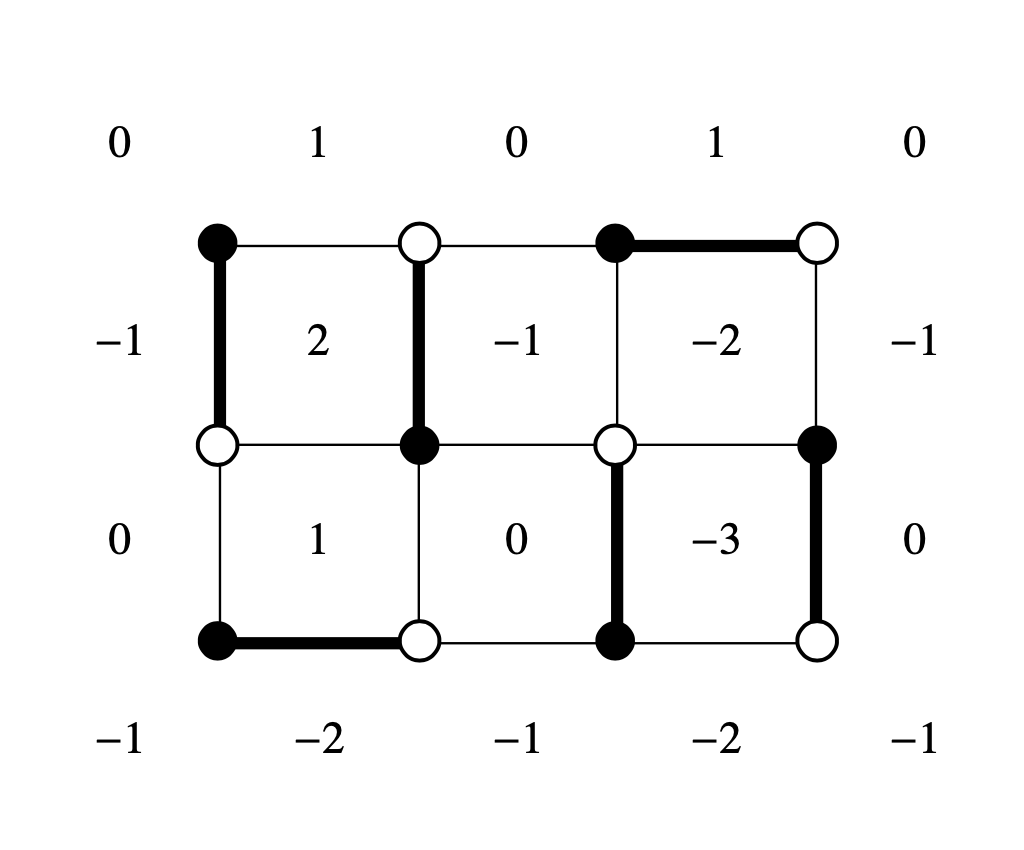
\includegraphics[width=0.4\hsize]{height.png}
    \end{figure}
    これは以下のように決める。
    \begin{itemize}
        \item 白を右に見て占有されている辺を横切ると高さは$+3$
        \item 白を右に見て占有されていない横切ると高さは$-1$
    \end{itemize}
\end{frame}
\begin{frame}{\currentname}
    ここで一つの白い頂点に対し、そのまわりの高さの平均は以下のようになる。
    \begin{figure}[H]
        \centering
        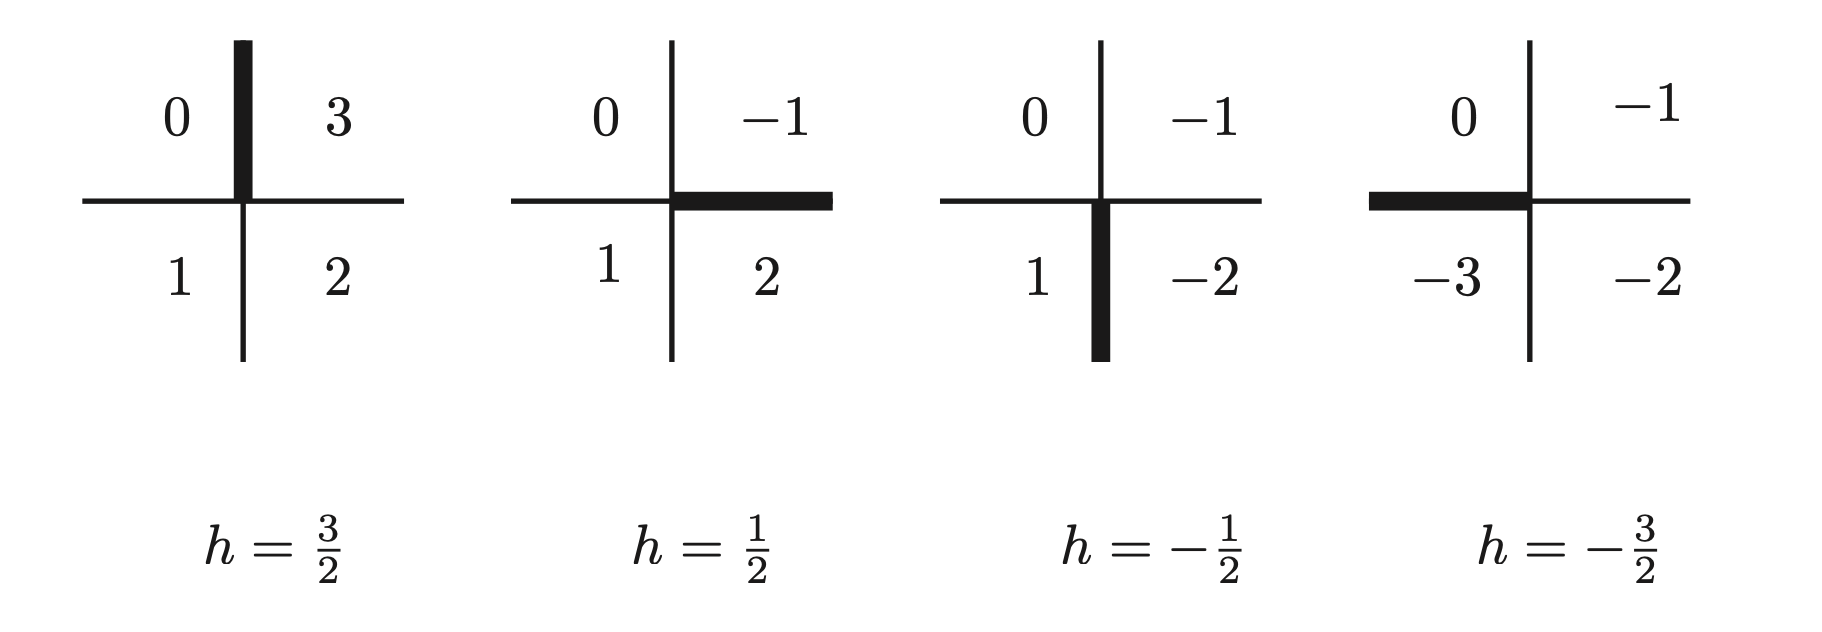
\includegraphics[width=0.7\hsize]{height_average.png}
    \end{figure}
    $h$の原点をずらすと、これらが$h = 0,1,2,3$に対応するようにできる。

    高さ関数をコンパクト化して角度変数$φ$を$φ = (𝜋/2)h$と定義する。
    ダイマーの密度と$φ$の対応は以下のようにして得られる。
    \begin{align}&
        n_x = ÷{1}{4} + ÷{1}{2𝜋}(-1)^{x+y}∂_yφ
            = (-1)^x\cosφ \\
            &
        n_y = ÷{1}{4} + ÷{1}{2𝜋}(-1)^{x+y+1}∂_xφ
            = - (-1)^y\sinφ   
    \end{align}
    (Fradkinはこれらを足してしまっているが、怪しい。)
\end{frame}
\begin{frame}{\currentname}
    $φ(𝒙)$に対する有効理論はfree bosonであり、作用は
    \begin{align}
        S[φ] = ∫\𝑑^2x ÷{K}{2}(∇φ(𝒙))²
    \end{align}
    である。
    free bosonに対して以下の演算子を考える。
    \begin{align}
        V_n(𝒙) = ℯ^{¡nφ(𝒙)},␣ \~V_m(𝒙) = ℯ^{¡mϑ(𝒙)}
    \end{align}
    ただし$ϑ$はCauchy-Riemannの関係式によって
    \begin{align}
        ∂_iϑ = ε_{ij}∂_jφ
    \end{align}
    と定める。charge-density wave は$V₁(𝒙)$に対応づけられ、$1,¡,-1,-¡$の値を取る。
    columnar order parameterは$V₂(𝒙)$に対応づけられ、$±1$の値を取る。

    厳密解によって、ダイマー密度の相関関数のべき依存性は$1/|𝒙-𝒚|²$となることが知られている。
    vertex operator の相関関数
    \begin{align}
        ⟨V₁(𝒙)V₋₁(𝒚)⟩ = ÷{1}{|𝒙-𝒚|^{2Δ₁}},␣Δ₁ = ÷{1}{4𝜋K}
    \end{align}
    と比較すると、自由なダイマー模型に対応する点として$K_\𝚞{free} = 1/4𝜋$を得る。
\end{frame}
\begin{frame}{\currentname}
    量子論に戻る。
    $φ(𝒙),Π(𝒙)$を正準共役な変数とする:
    \begin{align}
        [φ(𝒙),Π(𝒚)] = ¡δ²(𝒙-𝒚)
    \end{align}
    QDMの有効理論のハミルトニアンとして、
    \begin{align}
        H₀ = ∫\𝑑^2x[
            ÷{1}{2}Π(𝒙)²
            +÷{A}{2}(∇φ(𝒙))²
            +÷{κ²}{2}(∇²φ(𝒙))²
        ]
    \end{align}
    を考えよう。
    \begin{enumerate}
        \item $A > 0$のときは秩序相に対応する。
        \item $A = 0$のときは量子臨界点に対応する。
    \end{enumerate}
    それぞれについて見ていく。
\end{frame}
\begin{frame}{\currentname}
    まず$A>0$のとき、$[T] = [L]$である。
    ハミルトニアンを作用に直すと
    \begin{align}
        S₀ = ∫\𝑑^2x\𝑑{τ}[
            ÷{1}{2}(∂_τφ(𝒙))²
            +÷{A}{2}(∇φ(𝒙))²
            +÷{κ²}{2}(∇²φ(𝒙))²
        ]
    \end{align}
    である。次元解析すると$[φ] = [L^{-1/2}]$であり、
    $[(∇²φ)²] = [L^{-5}]$はirelevantである。
    高さ関数の周期性から、この作用に
    \begin{align}
        S_\𝚞{int} = ∫\𝑑^2x\𝑑{τ} g \cos(4φ)
    \end{align}
    という項を追加する。
    $S_\𝚞{int}$は$A>0$のときrelevantであり、作用に含める必要がある。
    くりこみによって$g$が大きくなるため、$A > 0$の相は$g$の強結合相によって記述される。
    有効理論の作用は
    \begin{align}
        S_\𝚞{eff} = ∫\𝑑^2x\𝑑{τ}[
            ÷{1}{2}(∂_τφ(𝒙))²
            +÷{1}{2}(∇φ(𝒙))²
            +÷{g}{√A}\cos(4φ(x))
        ]
    \end{align}
    である。ただし$τ → τ/√A,~ 𝒙 → √A𝒙$のようにスケールを取り直した。
    このとき$φ$は$\cos(4φ)$の底の1つにあり、
    $φ$の揺らぎはgappedとなって質量$m²_\𝚞{eff} ≈ 16g/√A$をもつ。
    この相はcolomner orderをもつ。
\end{frame}
\begin{frame}{\currentname}
    次に$A = 0$の場合を考える。
    この場合の作用は
    \begin{align}
        S_\𝚞{QLM} = ∫\𝑑^2x\𝑑{τ}[
            ÷{1}{2}(∂_τφ)²+÷{κ²}{2}(∇²φ)²
        ]
    \end{align}
    であり、これを量子Lifschitz模型と呼ぶことにする。
    次元解析をすると$[T] = [L²]$であり、$[φ] = [1]$である。
    摂動として、$S_\𝚞{int}$の他にmarginalな項
    \begin{align}
        S₄ = ∫\𝑑^2x\𝑑{τ}g₄(∇φ)⁴
    \end{align}
    を考えることができる。
    これはmarginaly irelevantではあるが、
    $A < 0$の場合に秩序相を安定化する。
    古典的に安定な$φ$の配位が$∇φ = 𝑸$のようにシフトするので、
    \begin{align}
        φ(𝒙) = 𝑸⋅𝒙
    \end{align}
    となる。$𝑸$はcolomnar stateの傾きを表している。
    $S_\𝚞{QLM}+S₄+S_\𝚞{int}$を最小化するように$𝑸$を決定すると
    \begin{align}
        |𝑸| = √{÷{|A|}{4g₄}}
    \end{align}
    となる。
\end{frame}
\begin{frame}{\currentname}
    摂動を加えない場合はくりこみに対して不安定であるが、
    この場合は臨界点として重要である。
    量子Lifshitz模型のハミルトニアンをゲージ理論の言葉で表現すると、
    \begin{align}
        H_\𝚞{QLM-gauge}
        = ÷{κ²}{2}‖\~∂E‖²+ ÷{1}{2}‖\~∂A‖²
        = ∫(÷{κ²}{2}𝑑E∧★𝑑E + ÷{1}{2}𝑑A∧★𝑑A)
    \end{align}
    となる。
    $E,A$は正準交換関係$[E(e),A(e')] = ¡(e,e')$を満たし、
    状態はゲージ不変性$∂E(v)|\Phys⟩ = 0$を満たすとする。
    ここで双対な理論に移り、$∂ ↔ \~∂$とする。
    \begin{align}
        E(e) = \~∂φ(e),␣ Π(v) = ∂A(v)
    \end{align}
    とすると、ゲージ不変性$\~∂E = 0$は直ちに成り立つ。
    また$φ(v),Π(v)$の間の交換関係は
    \begin{align}
        [φ(v),Π(v')] = ¡(v,v')
    \end{align}
    となる。ハミルトニアンを$φ,Π$を使って表示すると、
    \begin{align}
        H_\𝚞{QLM-gauge}
        = ÷{1}{2}‖Π‖² + ÷{κ²}{2}‖𝛥φ‖²
        = ∫(÷{1}{2}Π∧★Π + ÷{κ²}{2}𝛥φ∧★𝛥φ)
    \end{align}
    である。
\end{frame}
\begin{frame}{\currentname}
    電荷演算子は
    \begin{align}
        O_n(v) = ℯ^{¡n(γ_v,E)} = ℯ^{¡(∂γ_v,φ)}
        = ℯ^{¡nφ(v)}
    \end{align}
    である。
    磁荷演算子は
    \begin{align}
        ℯ^{¡m(\~γ_v,A)}
    \end{align}
    である。磁荷があるときのゲージ不変性は$\~∂E = mv$であり、
    \begin{align}
        E = \~∂φ + ℬ,␣ \~∂ℬ = mv
    \end{align}
    と表せる。するとハミルトニアンは
    \begin{align}
        H_\𝚞{QLM-gauge}
        = ÷{1}{2}‖Π‖² + ÷{κ²}{2}‖𝛥φ+∂ℬ‖²
    \end{align}
    となる。
\end{frame}
\begin{frame}{\currentname}
    ここでSchrödinger汎函数$Ψ[φ]≔⟨[φ]|Ψ⟩$を用いて考える。
    ハミルトニアンの作用は
    \begin{align}
        HΨ[φ] &= ∫\𝑑^2x[
            -÷{1}{2}\δ^2{}{φ(𝒙)}
            +÷{κ²}{2}(∇²φ(𝒙))²
        ]Ψ[φ] = EΨ[φ]\∅
        &
        = ∫\𝑑^2x÷{1}{2}{Q[φ],Q^†[φ]}Ψ[φ]
    \end{align}
    と書ける。ただし$Q^†[φ],Q[φ]$は生成消滅演算子であり、
    \begin{align}
        Q[φ]
        = ÷{1}{√2}[-\δ_{φ(𝒙)}+κ∇²φ(𝒙)]
    \end{align}
    と定義される。
    基底状態は、汎函数微分方程式$QΨ₀[φ] = 0$を解くことで
    \begin{align}
        Ψ₀[φ] = ÷{1}{√{Z₀}}\exp(-∫\𝑑^2x ÷{κ}{2}(∇φ(𝒙))²)
    \end{align}
    と求まる。
    ただし、
    \begin{align}
        Z₀ = ∫\𝒟{φ}\exp(-∫\𝑑^2xκ(∇φ(𝒙))²)
    \end{align}
    である。
    これは$K = 2κ$のfree bosonの分配関数になっている。
\end{frame}
\begin{frame}{\currentname}
    電荷演算子の相関関数は
    \begin{align}
        ⟨Ψ₀|O_{n₁}(𝒙₁)⋯O_{n_N}(𝒙_N)|Ψ₀⟩
        = ⟨V_{n₁}(𝒙₁)⋯V_{n_N}(𝒙_N)⟩_\𝚝{free boson}
    \end{align}
    となって、$K = 2κ$のfree bosonにおけるvertex operatorの相関関数に帰着する。
    vertex operatorのOPEは
    \begin{align}
        V_{n₁}(𝒙₁)V_{n₂}(𝒙₂) ∼ |𝒙₁-𝒙₂|^{n₁n₂/4𝜋κ}V_{n₁+n₂}(𝒙₂) + ⋯
    \end{align}
    であるから、これを繰り返し適用していけば相関関数は求まる。
    特に、
    \begin{align}
        ⟨V_{-n}(𝒙₁)V_{n}(𝒙₂)⟩ = |𝒙₁-𝒙₂|^{-n²/4𝜋κ}
    \end{align}
    であるから、電荷演算子$O_n$のスケーリング次元が
    \begin{align}
        Δ_n = {n²}{8𝜋κ}
    \end{align}
    となることが分かる。
\end{frame}
\begin{frame}{\currentname}
    次に磁荷演算子について考える。これは
    \begin{align}
        \~O_m(f) = ℯ^{2𝜋¡m(\~γ_f,A)}
        = ℯ^{2𝜋¡(α_f,Π)}
    \end{align}
    と表される。ただし、
    \begin{align}
        \~∂\~γ_f = f,␣
        \~∂α_v = m\~γ_v
    \end{align}
    である。よって$α_v$は$\~∂²α_v = mv$の解である。
    連続の言葉で書くと
    \begin{align}
        𝑑²α_𝒙(𝒚) = mδ²(𝒙-𝒚),␣
    \end{align}
    となる。一見すると左辺は$0$になるが、
    $ℯ^{2𝜋¡α_𝒙}$が一価になることのみを要請すれば、
    \begin{align}
        α_𝒙(𝒚) = m\arg(𝒚-𝒙)
    \end{align}
    という解がある。
    $Π$は$φ$に共役な演算子だったので、磁荷演算子は
    \begin{align}
        \~O_m(𝒙)|[φ]⟩ = |[φ-α_𝒙]⟩
    \end{align}
    という作用になっている。
    これは特異ゲージ変換とみなせる。
\end{frame}
\begin{frame}{\currentname}
    磁荷がある場合のSchrödinger汎函数は、
    \begin{align}
        Ψ_{m,𝒙}[φ]
        = ⟨[φ]|\~O_m(𝒙)|Ψ₀⟩
        = ÷{1}{√Z₀}\exp(-÷{κ}{2}‖\~∂φ-m\~γ_𝒙‖²)
    \end{align}
    となる。すると、$\~γ_𝒙$がゲージ場に見えてくる。
    磁荷演算子の相関関数は
    \begin{align}
        ⟨Ψ₀|\~O_{m₁}(𝒙)⋯\~O_{m_M}(𝒙_M)|Ψ₀⟩
        = ÷{1}{Z₀}∫\𝒟{φ}\exp(-κ∫\𝑑^2𝒙(∇φ-𝑨)²)
    \end{align}
    となる。
    ここでベクトルポテンシャル$𝑨$は
    \begin{align}
        ∇×𝑨(𝒙) = 2𝜋∑_{l=1}^M m_lδ²(𝒙-𝒙_l)
    \end{align}
    を満たす。
    磁荷演算子のスケーリング次元を求めるためには、
    シリンダー時空において、
    compactified free bosonの巻きつき数$m$の基底状態のエネルギーを求めればよい。
    詳細は省くが
    \footnote{
        Yellow book (6.94) で$n = 0,g = 2κ$とすると、$\~Δ_m = (L₀+\bar{L}₀)|0⟩$から求まる。
    }
    \begin{align}
        \~Δ_m = 2𝜋κm²
    \end{align}
    となる。
\end{frame}
\begin{frame}{\currentname}
    Green関数は
    \begin{align}
        G(𝒙-𝒙',τ-τ') = ⟨φ(𝒙,τ)φ(𝒙',τ')⟩\
        = ∫÷{\𝑑{ω}}{2𝜋}∫÷{\𝑑^2𝒒}{(2𝜋)²}
            ÷{ℯ^{¡ω(τ-τ')-¡𝒒⋅(𝒙-𝒙')}}{ω²+κ²(𝒒²)²}
    \end{align}
    となる。これを正則化して、
    \begin{align}
        G_\𝚞{reg}(𝒙,τ) ≔ G(𝒙,τ) - G(𝒂,0)
        ≔-÷{1}{8𝜋κ}[\ln(÷{𝒙²}{a²})+Γ(0,÷{𝒙²}{4κ|τ|})]
    \end{align}
    とする。(確かめてない。)
    $Γ(0,z)$は
    \begin{align}
        Γ(0,z) = ∫_z^∞÷{\𝑑{s}}{s}ℯ^{-s}
    \end{align}
    と定義される。漸近的な振る舞いは
    \begin{align}
        G_\𝚞{reg}(𝒙,τ) = \begin{cases}
            -(1/4𝜋κ)\ln(|𝒙|/a) & |t|  → 0\\
            -(1/8𝜋κ)\ln(4κ|τ|/a²𝛾) & |𝒙| → a
        \end{cases}
    \end{align}
    となる。ここで$\ln 𝛾 = 0.577$はEuler定数。
\end{frame}
\begin{frame}{\currentname}
    vertex operatorが正確には正規積をとったものであることに注意すると、
    Wickの定理から
    \begin{align}
        ⟨O_n(𝒙,τ)^†O_n(𝒙',τ')⟩
        = ℯ^{n²G_\𝚞{reg}(𝒙-𝒙',τ-τ')}
    \end{align}
    が成り立つ。よって、$|τ-τ'| → 0$のとき
    \begin{align}&
        ⟨O_n(𝒙,0)^†O_n(𝒙',0)⟩ = (÷{a}{|𝒙-𝒙'|})^{n²/(4𝜋κ)}
    \end{align}
    となる。また$|𝒙-𝒙'| → a$のとき
    \begin{align}
        ⟨O_n(𝟎,τ)^†O_n(𝟎,τ')⟩ = (÷{a²γ}{4κ|τ-τ'|})^{n²/(8𝜋κ)}
    \end{align}
    となる。
\end{frame}
\end{document}  